\chapter{具体需求}
% <The following sections must be repeated for each requirement. >

% 在每一条需求描述中重复下列部分
\section{功能需求}
% This section describes how the input of the software is translated to the output. It describes the essential action the software must perform.

% For each kind of function, or each independent function in some cases, the requirements of input, process and output must be described, which are usually organized with the following four subsections:

% 本子章节应描述软件产品的输入怎样被转换成输出。它描述了软件必须执行的基本动作。 

% 对每一类功能或有时对每一个单独的功能,必须描述输入、处理、输出方面的需求。这些通常以下面四个子段落来组织:
% \subsection{功能需求1}
% Please don't use "Functional Requirement(1)" as the title of the functional requirement. Name the functional requirements with a few simple words and a requirement ID.  For example:
% 
% R.INTF.CALC.001 Calculating expression
% 
% R.INTF.CALC.002 Print
% 
% Naming the requirement ID shall follow the Software Requirements Management Procedure (REP01)
% 
% 用需求编号加上简短词汇做为功能需求名,不要用“功能需求(1)”作为功能名,例如:R.INTF.CALC.001 计算表达式
% 
% R.INTF.CALC.002 打印
% 
% 需求编号规则按照软件需求管理规程(REP01)进行
% \subsubsection{介绍}
% <Itemize the detailed functional requirements associated with this feature. These are the software capabilities that must be present in order for the user to carry out the services provided by the feature.  Include how the project should respond to anticipated error conditions or invalid inputs. Requirements should be concise, complete, unambiguous, verifiable, and necessary. Use "TBD" as a placeholder to indicate when necessary information is not yet available. >
% 
% 逐条列出与本特性相关的功能需求。包括项目如何响应预期的错误输入,非法条件和无效输入。需求应该简明,完整,不含糊,可验证,必要的。 当需要的信息不确定的时候使用“待定”。
% \subsubsection{输入}
% This section consists of:
% A. Detailed description of all input data of the function, including:
% Source of input
% Quantify
% Measurement units
% Timing requirements
% Valid input range that contains the precision and tolerance
% B. Reference of interface specification or interface control document that are provided in proper place.
% 
% 本子段落应包含下列内容:
% 
% A. 对该功能所有输入数据的详细描述,包括:
% 
% 		输入来源
% 		数量
% 		度量单位
% 		时间要求
% 		包含精度和容忍度的有效输入范围
% 		
% B. 在适当的地方提供的对接口规格或接口控制文档的参考。
% \subsubsection{处理}
% Describes all the operations on the input data, and the process to get the output data, including the following specifications:
% A. Verification of input data
% B. Exact order of the operations, including the time sequene of each event.
% C. Response to exception, such as:
% 		 Overflow
% 		Communication failure
% 		Error process
% D. Any method used to transfer the input data to the output data. (such as equation,mathematic algorithm and logical operation)
% For example.
% 		The formula to calculate the income tax in a pay roll.
% 		the weather model used for weather forecast
% E. Verification of output data.
% 本子段落应描述对输入数据所执行的所有操作和如何获得输出的过程。这包括下列规格:
% 
% A. 输入数据的有效性检测。
% 
% B. 操作的确切次序,包括各事件的时序。
% 
% C. 对异常情况的回应,例如:
% 		溢出
% 		通信失败
% 		错误处理
% D. 用于把系统输入转换到相应输出的任何方法(诸如方程式,数学算法,逻辑操作)。例如,这可能描述下列方面:
% 		对工资单里代扣所得税的计算公式。
% 		用于气象预报的气象模型。
% 		
% E.	对输出数据的有效性检测。
% \subsubsection{输出}
% This section should include:
% A. The detailed description of output data of the function, including:
% 		Target to output to (Such as a printer or a file)
% 		Quantity
% 		Measurement units
% 		Time sequence
% 		Valid output range including the precision and tolerance
% 		Process of the invalid value.
% 		Error message.
% B. Reference of interface specification or interface control document that are provided in proper place.
% For the systems with their requirements focused on the input/output actions, all the important input/output actions and the time sequences of the input/output pairs should be described in the SRS. In a system that inputs and actions are memorized as the basis for the reactions to be taken, the timing sequence for the input/output pairs must be available here. This kind of functional action is similar to a status machine.  
% 本子段落应包含:
% 
% A. 对该功能所有输出数据的详细描述,这个描述包括:
% 		输出的到何处(如打印机,文件)
% 		数量
% 		度量单位
% 		时序
% 		包含精确度和容忍度的有效输出范围
% 		对非法值的处理
% 		错误消息
% 		
% B. 在适当的地方提供对接口规格或接口控制文档的参考。
% 
% 此外,对那些需求集中在输入/输出行为的系统,SRS应描述所有重要的输入/输出行为及输入输出对的次序。对一个需要记忆其行为以根据输入和过去的行为进行反应的系统,输入输出对的次序是要求的;这种功能行为就类似于有限状态机。

\subsection{R.INSTANT.MESSAGE.USERS.001 新用户注册}
\subsubsection{介绍}

账号注册,用户使用邮箱和密码新建账号。每位用户在注册时需要提供基本的用户信息(用作用户ID的邮箱,密码),和可选的用户资料(User Profile,如头像,性别,出生日期,所在地等)。

\subsubsection{输入}
\begin{itemize}
	\item 邮箱:可以接收邮件的合法邮箱
	\item 密码:由数字字母和特殊字符组成,三者均须出现,且至少为8位
	\item 确认密码:确保和密码一致
	\item (可选)用户资料:头像,性别,出生日期,所在地
	\item (可选)权限配置信息:
		\begin{enumerate}	
		\item 用户资料中的每个条目对自己好友是否可见
		\item 用户资料中的每个条目对陌生人是否可见
		\item 能否通过地理位置信息搜索到自己
		\end{enumerate}
	\end{itemize}

\subsubsection{处理}
\begin{enumerate}
	\item 检查邮箱是否合法
	\item 检查邮箱是否已被注册
	\item 检查密码是否和确认密码一致
	\item 检查密码强度是否合理
	\item 若用户上传了头像图片,检查该图片大小符合服务器上传文件大小限制
	\item 检查用户填写的其他用户资料值是否合法
	\item 将新用户记录插入数据库
	\end{enumerate}
若存在至少一项检查未通过,则本次操作失败;若所有检查均通过,则在数据库用户表中插入一条新记录,并根据输入信息填写字段值。

\subsubsection{输出}
在用户界面提示注册成功或失败。对于失败的操作需要提示出错原因(如数据项不合法、网络异常)。


\subsection{R.INSTANT.MESSAGE.USERS.002 变更自己的用户资料(User Profile)}
\subsubsection{介绍}
应允许用户在创建自己的帐号后,再次修改自己的用户资料。\\
{
	\color{red}
	为用户的隐私考虑,用户可配置自己用户资料各个字段的访问权限,原则上应包括:
	\begin{itemize}
		\item 该项对好友是否可见
		\item 该项对陌生人是否可见
	\end{itemize}
	(用户ID由于会被多个数据库表所引用,修改开销较大,故修改用户ID未列入需求。)
}


\subsubsection{输入}
\begin{itemize}
	\item 要修改的用户资料
	\item (可选)用户资料各字段的权限配置信息
	\item 当前用户所对应的ID(由客户端程序获得,无需用户输入)
	\end{itemize}

\subsubsection{处理}
检查修改后的用户资料是否合法,与R.INSTANT.MESSAGE.USERS.001中的检查步骤相同。
若存在至少一项检查未通过,则本次操作失败;若所有检查均通过,则在数据库用户表中修改已存在的记录,并根据输入信息填写字段值。
\subsubsection{输出}
在用户界面提示修改成功或失败。对于失败的操作需要提示出错原因(如数据项不合法、网络异常)。


\subsection{R.INSTANT.MESSAGE.USERS.003 使用用户ID查找用户资料(User Profile)}
\subsubsection{介绍}
用户可通过搜索另一用户的ID来访问另一个用户所公开的基本资料。
\subsubsection{输入}
\begin{itemize}
	\item 要查询的用户ID
	\end{itemize}
\subsubsection{处理}
在数据库内执行查询语句,若查找到相应用户,则返回该用户{\color{red}设置为公开访问权限的}用户资料项;若未查找到,本次操作失败。
\subsubsection{输出}
若操作成功,在用户界面显示相应的用户资料;若操作失败,返回相应的出错原因(如用户不存在、网络异常)。


\subsection{R.INSTANT.MESSAGE.USERS.004 通过地理位置发现周边的用户}
\subsubsection{介绍}
通过GPS或基站信号记录每位用户的大致或精确的位置,由服务器完成分析,并向每位用户推送距离该用户较近的50个用户的用户资料。\\
{\color{red}为用户的隐私考虑,用户可选择是否公开自己的位置信息。若用户选择不公开位置信息,该用户将不会被返回至搜索结果。}
\subsubsection{输入(由客户端自动完成)}
\begin{itemize}
	\item 用户ID
	\item 用户的位置信息(由客户端通过系统API获取)
\end{itemize}
\subsubsection{处理}
服务器端采用聚类算法,将处于相近地理位置的用户聚集至相同的一组,并将该组用户推送给组内的每一个用户。
\subsubsection{输出}
在每个用户的推送中显示与其距离相近的用户列表,及其用户资料。


\subsection{R.INSTANT.MESSAGE.USERS.005 申请好友}
\subsubsection{介绍}
用户均可以通过以上各种搜索和发现用户的方式,向别的用户发出添加好友的请求。合法的申请发出后,对方若同意申请,则双方的联系人列表中均会加入对方的条目。
\subsubsection{输入}
\begin{itemize}
	\item 对方用户ID(当用户通过搜索或别的方式查找到某一用户并申请好友时,此字段由客户端自动获得)
	\item 一段文本验证消息
\end{itemize}
\subsubsection{处理}
\begin{itemize}
	\item 当用户发出申请后,此申请会作为一条文本消息发送至对方。文本消息发送时的处理流程见“R.INSTANT.MESSAGE.CHAT.001 文本聊天”。
	\item 对方接收到该消息后,可选择同意申请或者拒绝申请。若对方忽略该消息足够长时间,系统默认会选择拒绝申请。
	\item 当对方同意申请后,检测两个用户已有的好友数量。若至少有一个用户的已有好友数量到达允许的最大值,则本次操作失败并返回;
	若两个用户的已有好友数量均未到达最大值,则在各自的联系人表中加入对方的记录。
\end{itemize}
\subsubsection{输出}
\begin{itemize}
	\item 当用户发出合法的申请后,在用户界面显示“请求已发送,等待对方审核”的提示消息。
	\item 当对方对申请给出回复后,在用户界面显示相应的提示。
	\item 当操作失败时(好友数量过多,或网络原因),在用户界面显示出错原因。
\end{itemize}

{
\color{red}
\subsection{R.INSTANT.MESSAGE.USERS.006 好友删除}
\subsubsection{介绍}
用户可以在客户端将自己的好友删除
\subsubsection{输入}
\begin{itemize}
	\item 对方用户ID
\end{itemize}
\subsubsection{处理}
客户端向用户再次确认后,会向服务器发送请求,服务器会将对应的记录从数据库上删除。
\subsubsection{输出}
\begin{itemize}
	\item 当操作成功时,在用户界面显示成功提示
	\item 当操作失败时(好友不存在,或网络原因),在用户界面显示出错原因。
\end{itemize}
\subsection{R.INSTANT.MESSAGE.USERS.007 好友推荐}
\subsubsection{介绍}
由服务端依据多个维度的数据定期推送可能认识的人至用户客户端。可从以下的多个维度查找合适的候选用户用于推送:
\begin{itemize}
	\item 与该用户处于相同城市的用户
	\item 与该用户有着类似的用户资料字段(如年龄、兴趣爱好)
	\item 与该用户同时处于多个聊天群组
	\item 与该用户同时与多个另外的用户是好友关系(即二度人脉)
\end{itemize}
\subsubsection{输入}
由服务端自动推送,无需用户输入。
\subsubsection{处理}
当服务器计算出可能认识的用户时,向客户端发送推送消息。客户端发出通知,并生成一个用户列表,每一个条目均包含一个申请好友的入口。
\subsubsection{输出}
\begin{itemize}
	\item 当服务器计算出可能认识的用户时,客户端显示推送消息,以及申请好友的入口。
	\item 当服务器未筛选出符合条件的用户时,客户度静默失败,不显示任何推送。
\end{itemize}

\subsection{R.INSTANT.MESSAGE.USERS.008 用户主页}
\subsubsection{介绍}
每位注册用户均可拥有该用户专属的灵活的、高度自定义的个人主页。\\
主页本质上为HTML静态网页,用户可从本地上传多个HTML/CSS文档或者JavaScript脚本来定制他们的主页。此外,考虑到广大用户的方便,客户端本身也应提供基本的网页模板和相应的生成、部署工具。\\
用户可配置该主页的访问权限,原则上应可选以下选项:
\begin{itemize}
	\item 允许Internet用户访问
	\item 仅允许用户好友访问
	\item 仅允许用户指定的好友访问
	\item 仅允许用户自己访问
\end{itemize}


\subsection{R.INSTANT.MESSAGE.USERS.009 好友清理}
\subsubsection{介绍}
客户端可依据各种不同的筛选条件,如最近的聊天时间、聊天频率等,筛选出部分不常联系的好友。用户可在筛选出的列表中实施部分或批量删除。
\subsubsection{输入}
由系统生成,无需用户输入。
\subsubsection{处理}
客户端会向服务器发送请求,服务器会将对应的多条记录从数据库上删除
\subsubsection{输出}
\begin{itemize}
	\item 当操作成功时,在用户界面显示成功提示
	\item 当操作失败时(好友不存在,或网络原因),在用户界面显示出错原因。
\end{itemize}

\subsection{R.INSTANT.MESSAGE.USERS.0010 设置黑名单}
\subsubsection{介绍}
用户可以在客户端将其他用户加入黑名单,黑名单中的用户不能再向自己申请好友,发起临时会话。
\subsubsection{输入}
\begin{itemize}
	\item 对方用户ID
\end{itemize}
\subsubsection{处理}
客户端会向服务器发送请求,服务器会在数据库上增加黑名单的记录
\subsubsection{输出}
\begin{itemize}
	\item 当操作成功时,在用户界面显示成功提示
	\item 当操作失败时(用户不存在,或网络原因),在用户界面显示出错原因。
\end{itemize}

\subsection{R.INSTANT.MESSAGE.USERS.0011 隐私设置}
\subsubsection{介绍}
用户可以在客户端进行设置,可设置能够通过何种方式添加好友,好友可以查看那些资料,陌生人可以查看那些资料,主页查看权限等
\subsubsection{输入}
\begin{itemize}
	\item 添加好友方式
	\item 好友权限
	\item 陌生人权限
\end{itemize}
\subsubsection{处理}
客户端会向服务器发送请求,服务器从表单中读取数据,并在数据库上修改对应的记录
\subsubsection{输出}
\begin{itemize}
	\item 当操作成功时,在用户界面显示成功提示。
	\item 当操作失败时,在用户界面显示出错原因。
\end{itemize}
}


\subsection{R.INSTANT.MESSAGE.CHAT.001 发送文本消息}
\subsubsection{介绍}
发送文本给指定用户

\subsubsection{输入}
\begin{itemize}
	\item 文本消息
	\item 目标用户ID或群组ID
\end{itemize}

\subsubsection{处理}
\begin{enumerate}
	\item 检查文本长度是否超出限制,如果超出限制,则本次操作失败。
	\item 将消息发送给指定用户或群组

	\end{enumerate}

\subsubsection{输出}
\begin{itemize}
	\item 若发送成功,在聊天界面显示消息。
	\item 若发送失败,仍在聊天界面显示消息,外加发送失败的标志和出错原因,并显示重试操作按钮。
	\end{itemize}
	

\subsection{R.INSTANT.MESSAGE.CHAT.002 发送语音消息}
\subsubsection{介绍}
用户可使用设备自带的录音功能录制一段语音消息,并发送至对方用户或群组。
\subsubsection{输入}
用户语音
\subsubsection{处理}
\begin{enumerate}
	\item 检查音频大小是否超出限制,如果超出限制,则本次操作失败。
	\item 将音频文件发送给指定用户
	\end{enumerate}
\subsubsection{输出}
\begin{itemize}
	\item 若发送成功,在聊天界面显示。
	\item 若发送失败,仍在聊天界面显示,外加发送失败的标志和出错原因,并显示重试操作按钮。
	\end{itemize}

	
\subsection{R.INSTANT.MESSAGE.CHAT.003 发送图片消息}
\subsubsection{介绍}
用户可向对方用户或群组发送包含图片的消息。图片的来源可以是本机、网络或客户端的收藏夹。

\subsection{R.INSTANT.MESSAGE.CHAT.004 创建聊天群组}
\subsubsection{介绍}
创建一个新的聊天群组
\subsubsection{输入}
\begin{itemize}
	\item 群组名称
	\item 群组介绍文字
\end{itemize}
\subsubsection{处理}
\begin{enumerate}
	\item 检查群组名称字符串是否合法
	\item 检查该用户所创建群的数量是否已达上限
	\item 检查群组介绍文字是否符合长度要求
\end{enumerate}
若检查出错,则本次操作失败。若检查成功,则在数据库中创建相应的群组条目,并返回其唯一的数字ID。
\subsubsection{输出}
\begin{itemize}
	\item 若操作成功,则在用户界面显示新创建的群聊ID
	\item 若操作失败(名称不合法,群数量上限等原因),在用户界面显示出错原因
\end{itemize}

\subsection{R.INSTANT.MESSAGE.CHAT.005 邀请用户加入聊天群组}
\subsubsection{介绍}
邀请一个用户加入一个聊天群组,被邀请用户须是用户的好友。
\subsubsection{输入}
\begin{itemize}
	\item 被邀请的用户ID
	\item 群组ID(由客户端获取,用户无需输入)
\end{itemize}
\subsubsection{处理}
\begin{enumerate}
	\item 检测该群组已有的用户数量,若已达到最大值,则本次操作失败并返回。
	\item 检查用户ID、群组ID有效性。
	\item 检查被邀请用户是否是邀请者的好友。
	\item 若所有检查均通过,将邀请消息发送至被邀请的用户。否则本次操作失败。
	\item 对方接收到该邀请后,可选择同意邀请或者拒绝邀请。若对方忽略该消息足够长时间,系统默认会选择拒绝邀请。
	\item 将邀请结果回复给原用户。
\end{enumerate}
\subsubsection{输出}
\begin{itemize}
	\item 当用户发出合法的邀请后,在用户界面显示“请求已发送,等待对方审核”的提示消息。
	\item 当对方对邀请给出回复后,在用户界面显示相应的提示。
	\item 当操作失败时(好友数量过多,或网络原因),在用户界面显示出错原因。
\end{itemize}

\subsection{R.INSTANT.MESSAGE.CHAT.006 退出聊天群组}
\subsubsection{介绍}
解除用户与某聊天群组的关系。若该用户为群主,则用户在退出前须指定另一个成员作为新群主。
\subsubsection{输入}
群组ID(由客户端获取,用户无需输入)
\subsubsection{处理}
\begin{enumerate}
	\item 检查该用户是否为群主,如果是,则指引完成新群主的分配工作。
	\item 在数据库中执行相应的删除操作。
	\item 若当前群组的人数为0,在数据库中删除该群组本身。
\end{enumerate}
\subsubsection{输出}
在用户界面提示操作成功或失败。对于失败的操作需要提示出错原因(如网络异常)。
\subsection{R.INSTANT.MESSAGE.CHAT.007 解散聊天群组}
\subsubsection{介绍}
解散一个聊天群主。操作者须为群主。
\subsubsection{输入}
群组ID(由客户端获取,用户无需输入)
\subsubsection{处理}
\begin{enumerate}
	\item 检查操作用户是否为群主,若否,本次操作失败。
	\item 在数据库执行相应的删除操作。
\end{enumerate}
\subsubsection{输出}
在用户界面提示操作成功或失败。对于失败的操作需要提示出错原因(如网络异常,权限不足)。
\subsection{R.INSTANT.MESSAGE.CHAT.008 视频聊天}

\begin{figure}[h]
	\centering
	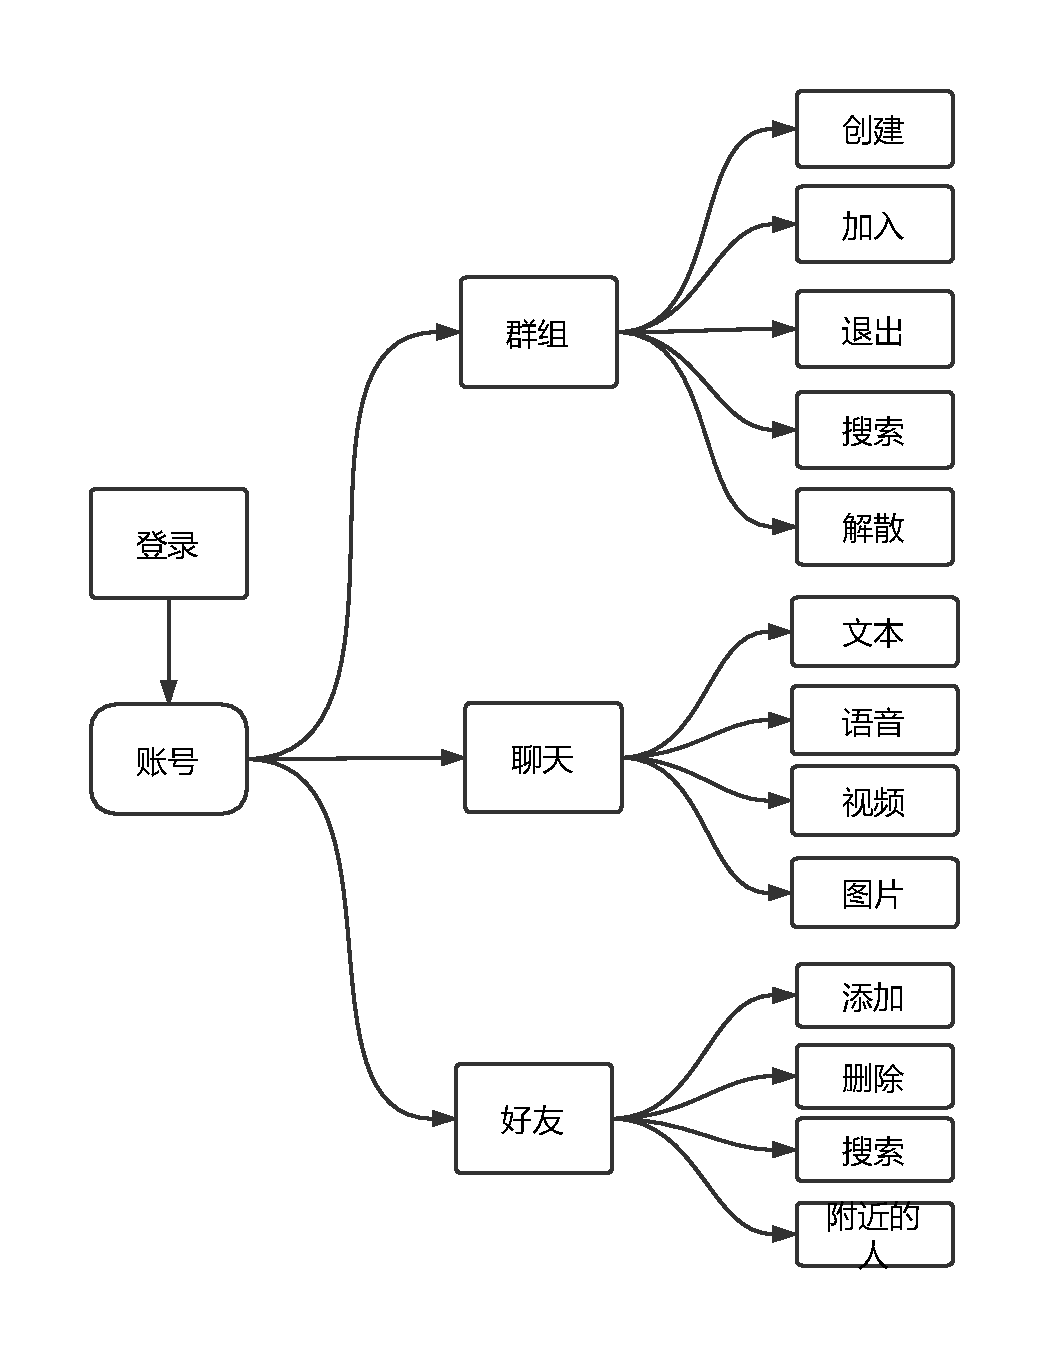
\includegraphics[width=10cm]{function}
	\caption{功能图} \label{fig:function}
\end{figure}

\section{性能需求}
% <If there are performance requirements, state them here and explain their rationale, to help the developers understand the intent and make suitable design choices. Specifies the timing relationships for real time systems. Such requirements should be made as specific as possible. >

% 如果有性能方面的需求,在这里列出并解释他们的原理。以帮助开发者理解意图以做出正确的设计选择。在实时系统中的时序关系。保证需求尽可能的详细而精确。
% \subsection{性能需求1}
% Describes the statically and dynamically quantized requirements on the software (or the interaction between user and the software)
% Static quantized requirement could include:
% A. Maximum number of terminal supported.
% B. Maximum number of users that can use the software at the same time.
% C. Maximum number of files and records to be processed
% D. Maximum size of  tables and files
% Dynamically quantized requirements could include:
% A. Specific duration of normal value and peak value of workload (e.g., one hour)
% B. Number of event and task and data volume to be processed 
% All these requirements should be described by measurable term, for example, saying "95% of the events should be processed in 1 second", instead of saying "the operator need not wait for the business to complete."
% Note: The quantized constraint of a detailed requirement should be described in the subsection of the detailed requirement.
% 本子章节应从整体上描述静态和动态的量化的对软件(或人与软件交互)的需求。
% 
% 静态的量化需求可能包括:
% 
% A. 支持的终端数目。
% 
% B. 支持的同时使用的用户数目。
% 
% C.处理的文件和记录的数目。
% 
% D.表和文件的大小。
% 
% 动态的量化需求可能包括:
% 
% A. 在正常和峰值工作量条件下特定时间段(如一小时)
% 
% B. 处理的事务和任务的数目以及数据量。
% 
% 所有的这些需求应以可测量的术语进行描述,例如所有的操作应在1秒内被处理完成,而不是描述成操作员不必等待操作的完成。
% 
% 注意: 用于一个具体功能的量化限制通常在该功能的处理子章节中描述。

\subsection{实时性需求}

系统应采用推送技术实现聊天消息的实时性。如 android 客户端可以使用 google 或小米等的推送平台,web app可以使用 websocket 长连接。

\subsection{并发性需求}

服务端应采用一定的技术实现高并发,保证在用户数量较大时仍能正常运行。
要求服务器至少能同时支持10000个客户端同时在线。

\section{外部接口需求}
\subsection{用户接口}
% <The interface of the system with the User and vice versa should be explained in detail. >
% 
% 详细描述系统与用户之间的接口
% 
% This section should include:
% A. Features that must be supported by the software for eachman-machine interface. For example, if the user operates from a display terminal, then the following should be included:
% 		Screen format required
% 		Page layout and content of report and menu
% 		Timing sequence for input and output
% 		Usage of some functional key combinations
% B. Every aspect about the use of the system's user interface. It could be a list that shows the user what should do and what should not do.  For example, an option of overlong or overshort message. . And same as other requirements, these requirements should be easily verified. For example, saying "A level 4 typist can finish function X in Z minutes after a one-hour training." instead of "A typist can finish function X"	
% 
% 这应描述下述内容:
% 
% A. 对每种人机界面,软件所必须支持的特性。例如,如果系统用户通过一个显示终端进行操作,那么应包含下述内容:
% 要求的屏幕格式
% 页面规划及报告或菜单的内容
% 输入和输出的相关时序
% 一些组合功能键的用法
% 
% B. 与系统用户接口使用相关的所有方面。这可能只是一个简单的关于系统怎样展示给用户而该做什么和不该做什么的列表。例如提供关于长或短错误消息选项。和所有其它需求一样,这些需求也应能被检验,例如,四级打字员经一小时的培训后能在Z分钟内完成功能X,而不是一个打字员能完成功能X。


\subsubsection{登录界面}

\begin{figure}[h]
	\centering
	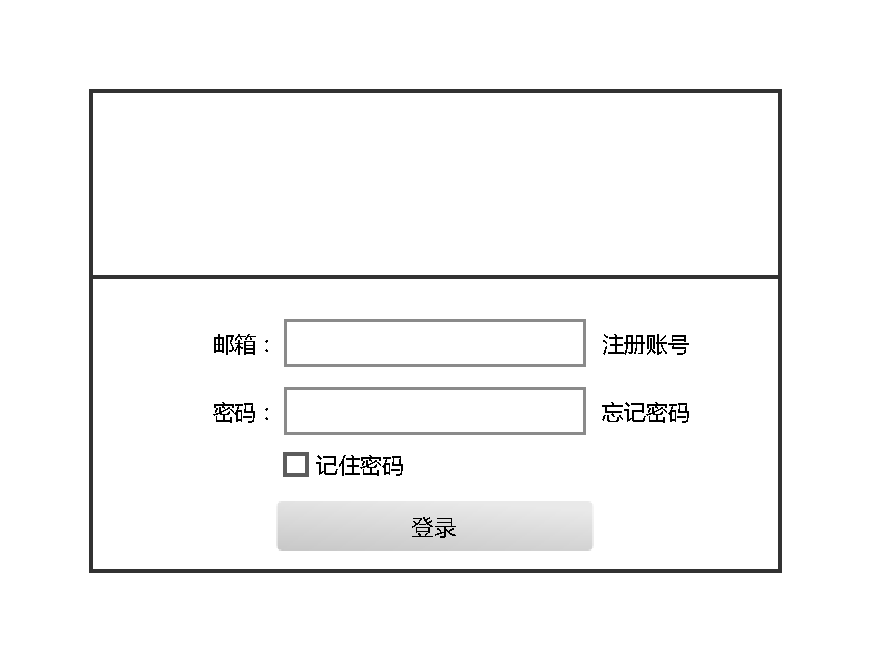
\includegraphics[width=13cm]{login_ui}
	\caption{登录界面} \label{fig:login_ui}
\end{figure}


如图 3.1。
输入邮箱密码登陆,可选择记住密码,右侧有注册账号和忘记密码的按钮。
界面上方放置banner图片,增加美观。

\clearpage
\subsubsection{主界面}
\begin{figure}[h]
	\centering
	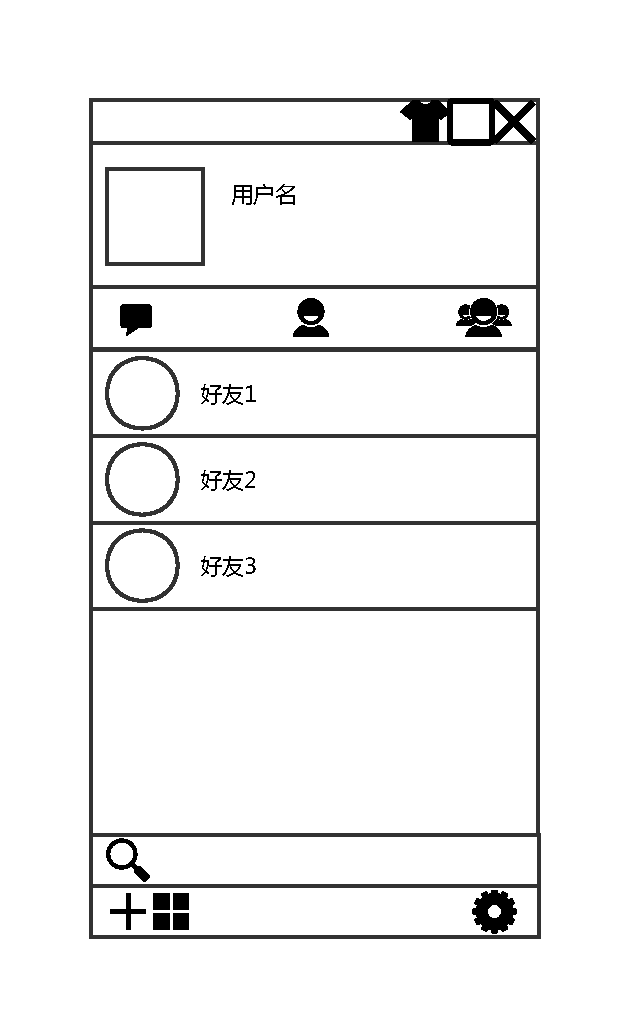
\includegraphics[width=10cm]{main_ui}
	\caption{主界面} \label{fig:main_ui}
\end{figure}

如图 3.2。
最上方显示自己的头像和用户名。
中间有三个标签页,从左到右分别是会话,好友和群组。
下方有一个搜索框,可用于搜索已添加的好友。
最下方的三个按钮的功能分别是添加新好友,菜单和设置。

\clearpage
\subsubsection{聊天界面}
\begin{figure}[h]
	\centering
	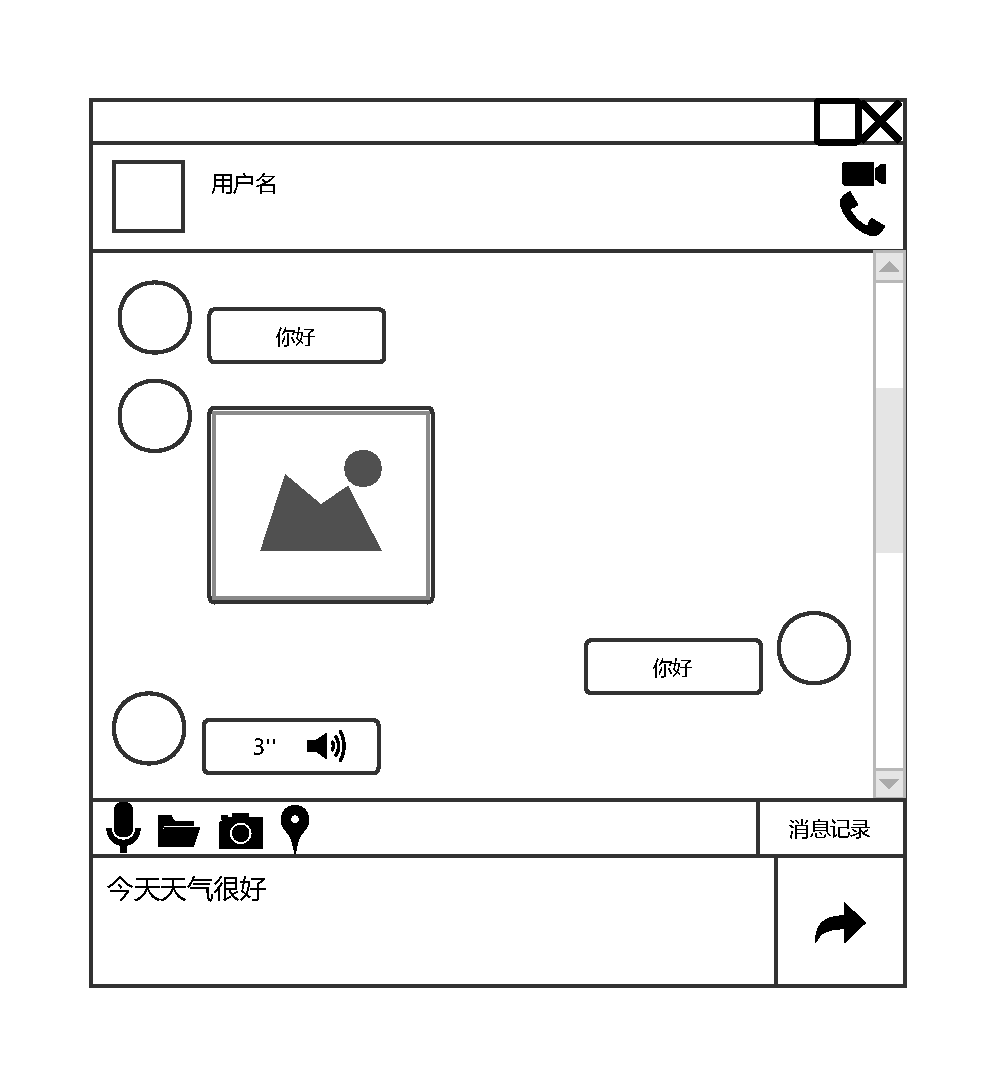
\includegraphics[width=10cm]{chat_ui}
	\caption{聊天界面} \label{fig:chat_ui}
\end{figure}


如图 3.3。
最上方显示对方的头像和用户名(或群的头像和群名),左侧可以开启视频或语音聊天。
中间为消息显示区,消息放在气泡中显示,自己的消息在右侧,其他人的在左侧。
最下方为文本输入框,左侧为发送按钮。
输入框上方为工具栏,可以用于发送图片和语音消息,可以查看聊天记录。

\subsubsection{用户搜索界面}
\begin{figure}[h]
	\centering
	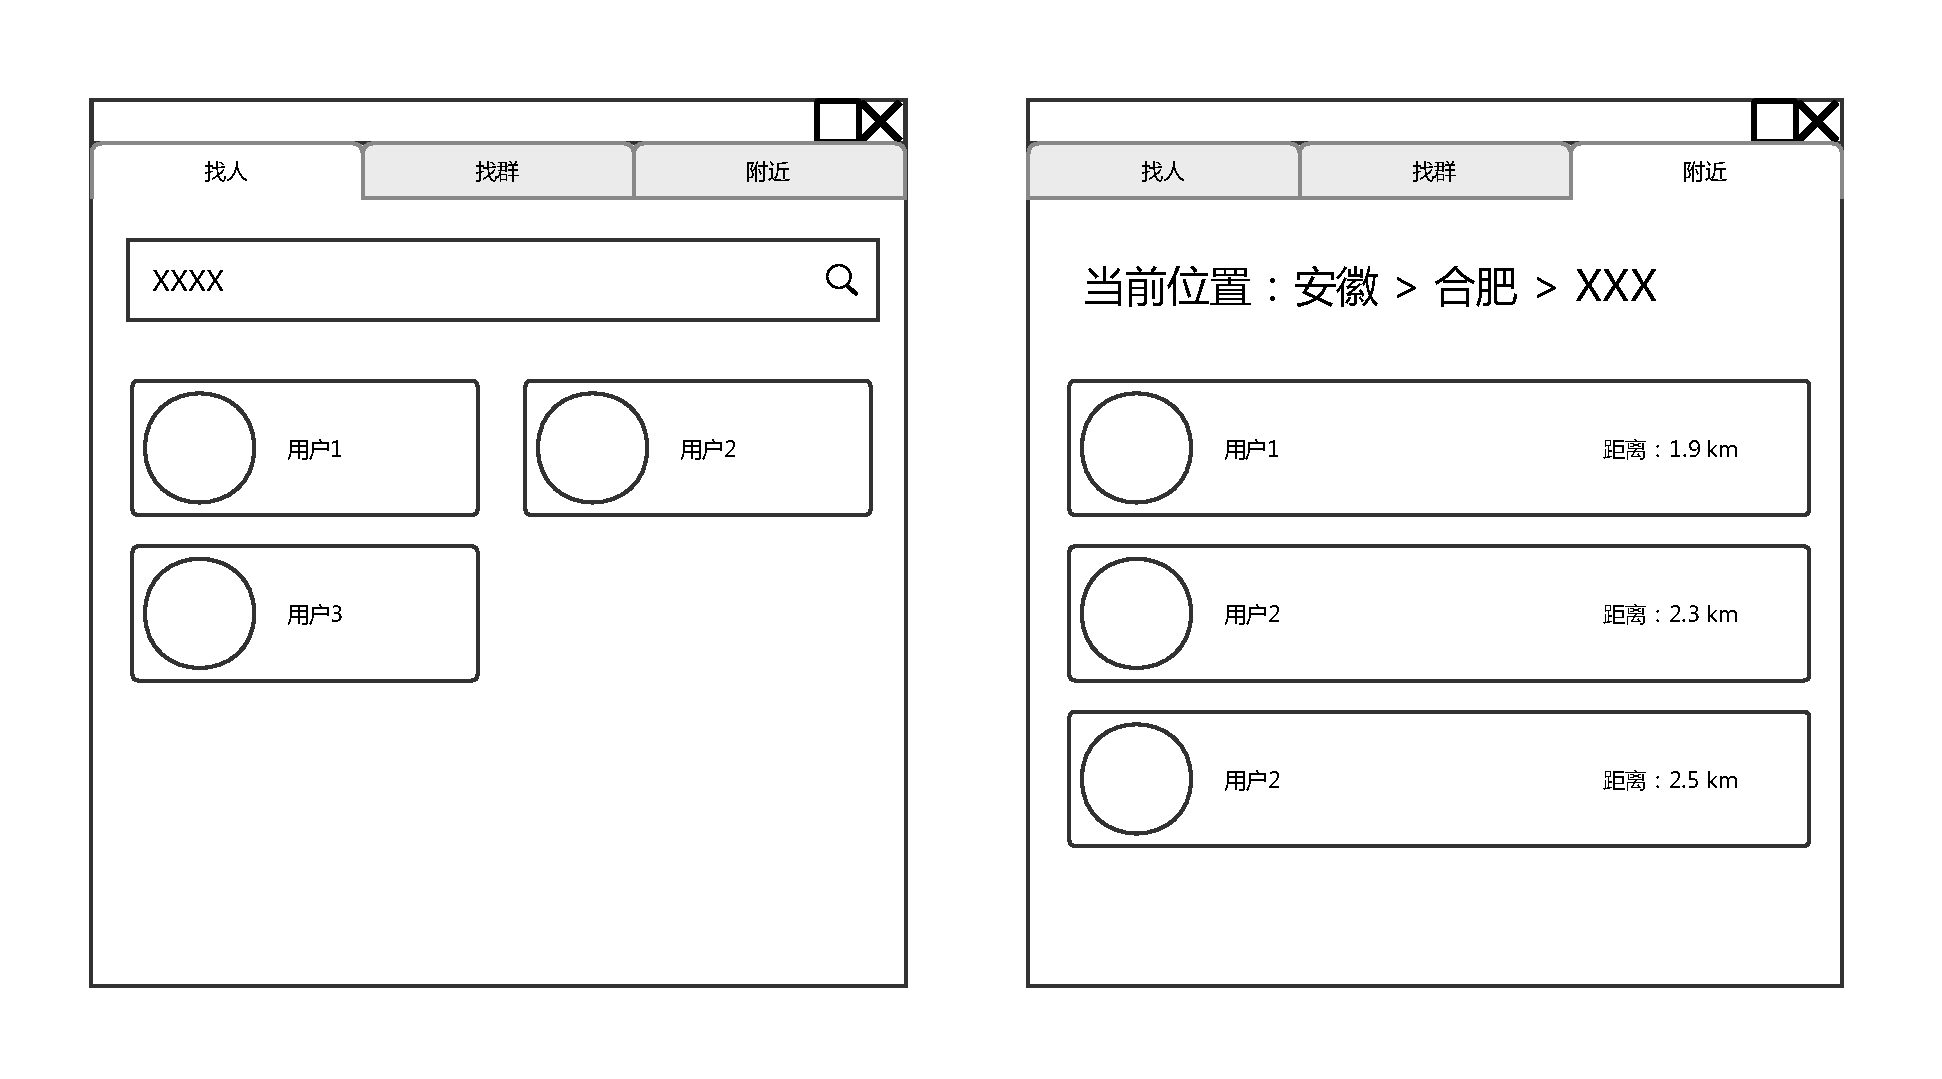
\includegraphics[width=10cm]{search_friend_ui}
	\caption{用户搜索界面} \label{fig:search_friend_ui}
\end{figure}

如图 3.4。
共三个标签页可用于搜人,搜群,附近。
找人,找群标签页在搜索框输入内容后显示结果。
附近标签页显示了当前位置和附近的用户以及估计的距离。
点击用户弹出用户信息界面

\begin{figure}[ht]
	\centering
	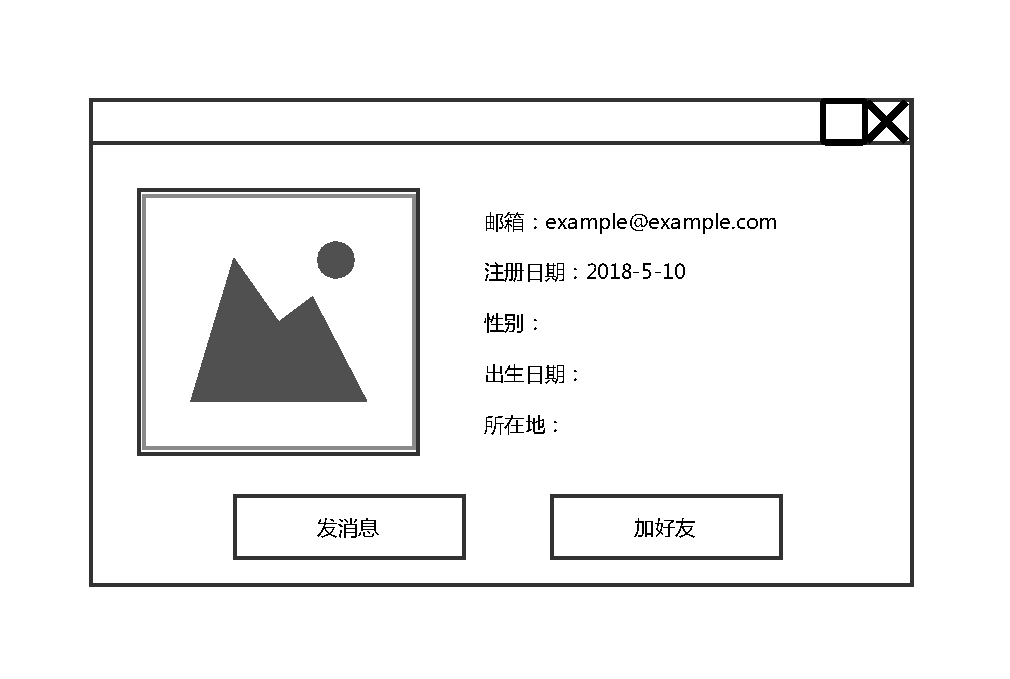
\includegraphics[width=15cm]{userinfo_ui}
	\caption{用户信息界面} \label{fig:userinfo_ui}
\end{figure}


\subsection{软件接口}
% <The interface with other system/modules/projects should be explained in detail. >
% 
% 详细描述与其他系统 /模块 /项目之间的接口
% 
% Describes how to use the other (required) software products. (such as data management system, operation system, or algorithm tools package), and the interfaces to other application systems (such as interfaces between the protocol process system and the database management system )
% For each required software product, following information should be provided:
% A. Name
% B. Mnemonic symbol
% C. Version number
% D. Source
% For each interface, this section should:
% A. Discuss the objective of the required software.
% B. Define the interfaces by content and format of message/function. If the interfaces have been clearly described in other documents, it is not necessary to describe in detail here. But the reference of those documents should be given.
% 
% 在此应描述如何使用其它(必需的)软件产品(例如,数据管理系统,操作系统,或算法工具包),以及与其它应用系统的接口(例如,协议处理系统和数据库管理系统之间的接口)。
% 
% 对每个必需的软件产品,应提供下列信息:
% A.	名字
% B.	助记符
% C.	版本号
% D.	来源
% 
% 对每个接口,本部分应:
% 
% A .	讨论与本软件产品相关的接口软件的目的。
% 
% B.	按消息/函数内容和格式定义接口。如果接口已在其它文档中很清楚地描述,就没有必要在这儿进行详细描述,但需说明应参考的文档。

% ython version > 3.5
% mysql version > 5.7

\subsection{硬件接口}
% <The interface with other hardware components should be explained in detail. >
% 
% 详细描述与硬件的接口
% 
% Describes the logical features of the interface between the software and hardware components, including the equipment supported and how the equipment and protocol is supported. 
% 
% Defines the interfaces according to the content and format of the software/hardware protocol. If the interfaces have been clearly described in other documents, it is not necessary to describe in detail here. But the reference of those documents should be given.
% 
% 在此描述软件产品和系统硬件组件之间接口的逻辑特征,也包括支持哪些设备、怎样支持这些设备和协议等。
%  
% 按软/硬件协议内容和格式定义接口。如果接口已在其它文档中很清楚地描述,就没有必要在这儿进行详细描述,但需说明应参考的文档。

部分平台的客户端需要使用录音设备获取音频输入,使用摄像设备获取视频输入,使用定位设备获取位置信息。

详细硬件接口设计见设计文档。

\subsection{通讯接口}
% <This should specify the various interfaces to communications such as local network protocols, etc.>
% 
% 详细描述通讯接口,如本地网络协议等。
% 
% Defines the interfaces according to the content and format of the message/function. If the interfaces have been clearly described in other documents, it is not necessary to describe in detail here. But the reference of those documents should be given.
% 
% 按消息/函数内容和格式定义接口。如果接口已在其它文档中很清楚地描述,就没有必要在这儿进行详细描述,但需说明应参考的文档。

客户端需要通过互联网和服务端通信,会使用到 Socket 通信和 HTTP 协议。

详细的通信接口设计见设计文档。